\begin{frame}
    \frametitle{Un poco de Historia}
    
    La primera aparición de la palabra robot es utilizada por Karl Capek en 1921 en su obra teatral R. U. R. (Rossum's Universal Robots). La palabra robot viene de la palabra checa \emph{robota} que significa esclavo.
    
    \TODO{agregar imagen obra de teatro wikipedia.}
    
    \note{
        Fuente: https://cs.stanford.edu/people/eroberts/courses/soco/projects/1998-99/robotics/history.html\\
        La obra teatral trata sobre una empresa que construye humanos artificiales orgánicos con el fin de aligerar la carga de trabajo del resto de personas. Aunque en la obra a estos hombres artificiales se les llama robots, tienen más que ver con el concepto moderno de androide o clon. Se trata de criaturas que pueden hacerse pasar por humanos y que tienen el don de poder pensar. Pese a ser creadas para ayudar a la humanidad, más adelante estas máquinas entrarán en confrontación con la sociedad, iniciando una revolución que acabará destruyendo la humanidad.}
\end{frame}

\begin{frame}
    \frametitle{Un poco de Historia}
    
    La palabra \emph{robotics} también fue utilizada por primera vez por Issac Asimov en 1942 en su cuento corto \emph{Runaround} (en español Circuito Vicioso).
    
    Primera Ley
    Un robot no hará daño a un ser humano ni, por inacción, permitirá que un ser humano sufra daño.
    Segunda Ley
    Un robot debe cumplir las órdenes dadas por los seres humanos, a excepción de aquellas que entren en conflicto con la primera ley.
    Tercera Ley
    Un robot debe proteger su propia existencia en la medida en que esta protección no entre en conflicto con la primera o con la segunda ley.
    
    \note{The word robotics was also coined by a writer.  Russian-born American science-fiction writer Isaac Asimov first used the word in 1942 in his short story Runabout.  Asimov had a much brighter and more optimistic opinion of the robot's role in human society than did Capek.  He generally characterized the robots in his short stories as helpful servants of man and viewed robots as a better, cleaner race.  Asimov also proposed three "Laws of Robotics" that his robots, as well as sci-fi robotic characters of many other stories.}
\end{frame}

\begin{frame}
    \frametitle{¿Qué es un Robot?}
    \note{hay varias definiciones.\\
        Fuente: https://robots.ieee.org/learn/what-is-a-robot/}
    
    Según Robot Institute of America, 1979
    Un manipulador reprogramable y multifuncional diseñado para mover material, piezas, herramientas o dispositivos especializados a través de varios movimientos programados para el desempeño de una variedad de tareas.
    
    Según la RAE
    Máquina o ingenio electrónico programable que es capaz de manipular objetos y realizar diversas operaciones.
    
    Una definición que usamos (https://robots.ieee.org/learn/what-is-a-robot/):
    Un robot es una máquina autónoma capaz de sensar su entorno, realizar cálculos para tomar decisiones y realizar acciones en el mundo real.
    
    \note{}
\end{frame}

\begin{frame}
    \frametitle{¿Qué es la Robótica?}
    La robótica es la intersección de la ciencia, la ingeniería y la tecnología que produce máquinas, llamadas robots, que sustituyen (o replican) las acciones humanas.
\end{frame}

\begin{frame}
    \frametitle{Aplicaciones de la Robótica}
%    \begin{figure}[!h]
%        \centering
%        \subfloat[] 
%        {
%            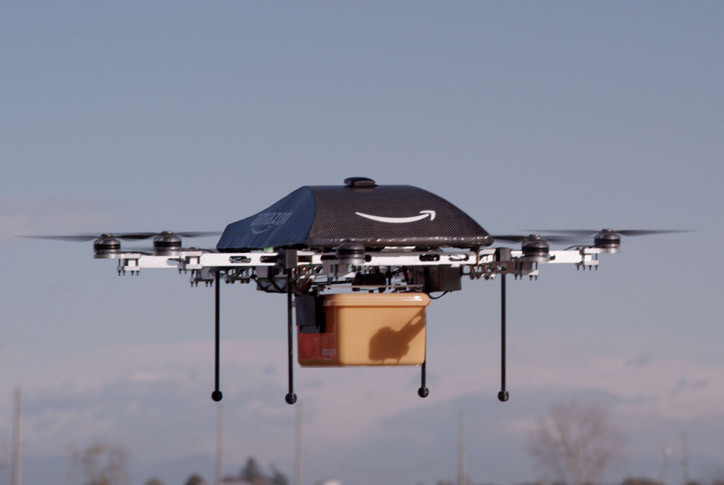
\includegraphics[width=0.33\columnwidth]{./images/introduction/drone.jpg}
%        }
%        \subfloat[] 
%        {
%            \includegraphics[width=0.33\columnwidth]{./images/introduction/GoogleCar.jpg}
%        }
%        \subfloat[] 
%        {
%            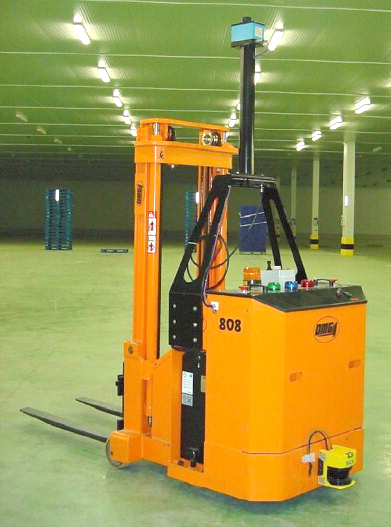
\includegraphics[width=0.16\columnwidth]{./images/introduction/industrial_robot.png}
%        }\\
%        \subfloat[] 
%        {
%            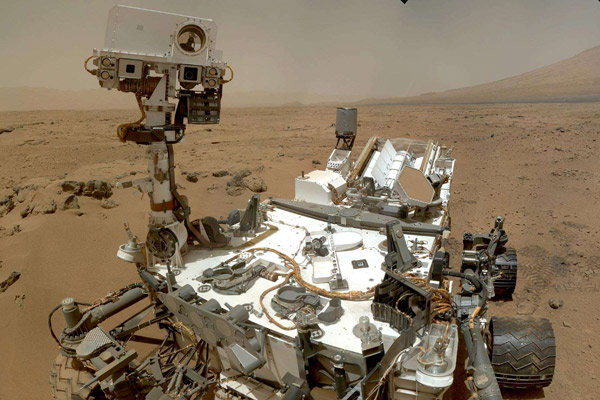
\includegraphics[width=0.33\columnwidth]{./images/introduction/curiosity.png}
%        }
%        \subfloat[] 
%        {
%            \includegraphics[width=0.33\columnwidth]{./images/introduction/hortibot.png}
%        }
%        \subfloat[]
%        {
%            \includegraphics[width=0.33\columnwidth]{./images/introduction/aqua2.png}
%        }		 
%    \end{figure}
\end{frame}

\begin{frame}
    \frametitle{Navegación autónoma}
    \begin{block}{}
        La navegación autónoma puede definirse a grandes rasgos como la capacidad de moverse de forma segura a lo largo de una trayectoria entre un punto de inicio y uno final [1].
    \end{block}
    \vspace{5mm}
    \begin{columns}
        \column{0.4\textwidth}
        \hspace{13pt}Pregunta:
        \begin{enumerate}
            \visible<2-7>{ \item[-] ¿Dónde estoy?}
            \visible<4-7>{\item[-] ¿Por dónde estoy yendo?}
            \visible<6-7>{\item[-] ¿Cómo llego hasta allí?}
        \end{enumerate}
        \column{0.6\textwidth}
        Respuesta:
        \begin{enumerate}[$\rightarrow$]
            \visible<3-7>{ \item  Cálculo de la posición (Localization)}
            \visible<5-7>{ \item  Representación del entorno (Mapping)}
            \visible<7-7>{\item  Planeamiento de movimiento (Motion planning)}
        \end{enumerate}
    \end{columns}
    \only<4>{}
    \vfill
    \begin{tiny}
        [1] J. J. Leonard - et al., ``Mobile robot localization by ...,'' IEEE Transactions on Robotics and Automation, 2002.
    \end{tiny}
\end{frame}